\section{Getting Started}

\subsection{Welcome}

Welcome to Variate Generator library! 

By the time you have read through this tutorial, you will be able to play with it.

\subsection{Compilation Enviroment Requirement}

As some C++11\footnote{Features such as lambda functions, variadic template and keyword auto, see http://www.open-std.org/jtc1/sc22/wg21/ for more information.} features are employed when implementing this library, 
before we get further, please check your compiler for C++11 compatablity.

\subsection{A Quick Example}

The code listed in Table \ref{code:gauss} shows how to generate gaussian random numbers:

\begin{small}
\begin{ttfamily}

\begin{center}
\rowcolors{1}{codeback1}{codeback2}
%\rowcolors{1}{White}{Silver}
%\begin{tabular}{|l|}
\begin{longtable}{|l|}
\caption{Source Code for a Gaussian Variate Example} \\
\label{code:gauss} \\
%%code
\hline
%\noindent
\mbox{}\textbf{\textcolor{RoyalBlue}{\#include}}\ \texttt{\textcolor{Red}{\textless{}vg.hpp\textgreater{}}} \\
%\mbox{} \\
\mbox{}\textbf{\textcolor{RoyalBlue}{\#include}}\ \texttt{\textcolor{Red}{\textless{}cmath\textgreater{}}} \\
\mbox{}\textbf{\textcolor{RoyalBlue}{\#include}}\ \texttt{\textcolor{Red}{\textless{}map\textgreater{}}} \\
\mbox{}\textbf{\textcolor{RoyalBlue}{\#include}}\ \texttt{\textcolor{Red}{\textless{}iostream\textgreater{}}} \\
%\mbox{} \\
\mbox{}\textcolor{ForestGreen}{int}\ \textbf{\textcolor{Black}{main}}\textcolor{BrickRed}{()} \\
\mbox{}\textcolor{Red}{\{} \\
\mbox{}\ \ \ \ \textit{\textcolor{Gray}{//generate\ double\ precision\ gaussian\ random\ numbers}} \\
\mbox{}\ \ \ \ \textit{\textcolor{Gray}{//using\ mt19937\ as\ random\ generator\ engine\ with\ arguments\ (0,4)}} \\
\mbox{}\ \ \ \ vg\textcolor{BrickRed}{::}\textcolor{TealBlue}{variate$\_$generator\textless{}double,\ vg::gaussian,\ vg::mt19937\textgreater{}}\ \textbf{\textcolor{Black}{vg}}\textcolor{BrickRed}{(}\textcolor{Purple}{0}\textcolor{BrickRed}{,}\ \textcolor{Purple}{4}\textcolor{BrickRed}{);}\ \ \ \  \\
\mbox{}\ \ \ \ std\textcolor{BrickRed}{::}\textcolor{TealBlue}{map\textless{}\ int,\ int\ \textgreater{}}\ sample\textcolor{BrickRed}{;} \\
%\mbox{} \\
\mbox{}\ \ \ \ \textit{\textcolor{Gray}{//generate\ 500\ gaussian\ numbers\ and\ store\ them\ in\ a\ map}} \\
\mbox{}\ \ \ \ \textbf{\textcolor{Blue}{for}}\ \textcolor{BrickRed}{(}\ \textbf{\textcolor{Blue}{auto}}\ i\ \textcolor{BrickRed}{=}\ vg\textcolor{BrickRed}{.}\textbf{\textcolor{Black}{begin}}\textcolor{BrickRed}{();}\ i\ \textcolor{BrickRed}{!=}\ vg\textcolor{BrickRed}{.}\textbf{\textcolor{Black}{begin}}\textcolor{BrickRed}{()+}\textcolor{Purple}{500}\textcolor{BrickRed}{;}\ \textcolor{BrickRed}{++}i\ \textcolor{BrickRed}{)} \\
\mbox{}\ \ \ \ \ \ \ \ sample\textcolor{BrickRed}{[}std\textcolor{BrickRed}{::}\textbf{\textcolor{Black}{round}}\textcolor{BrickRed}{(*}i\textcolor{BrickRed}{)]++;} \\
%\mbox{} \\
\mbox{}\ \ \ \ \textit{\textcolor{Gray}{//show\ the\ number\ generated}} \\
\mbox{}\ \ \ \ \textbf{\textcolor{Blue}{for}}\ \textcolor{BrickRed}{(}\ \textbf{\textcolor{Blue}{auto}}\ i\ \textcolor{BrickRed}{=}\ sample\textcolor{BrickRed}{.}\textbf{\textcolor{Black}{begin}}\textcolor{BrickRed}{();}\ i\ \textcolor{BrickRed}{!=}\ sample\textcolor{BrickRed}{.}\textbf{\textcolor{Black}{end}}\textcolor{BrickRed}{();}\ \textcolor{BrickRed}{++}i\ \textcolor{BrickRed}{)} \\
\mbox{}\ \ \ \ \textcolor{Red}{\{} \\
\mbox{}\ \ \ \ \ \ \ \ std\textcolor{BrickRed}{::}cout\ \textcolor{BrickRed}{\textless{}\textless{}}\ \textcolor{BrickRed}{(*}i\textcolor{BrickRed}{).}first\ \textcolor{BrickRed}{\textless{}\textless{}}\ \texttt{\textcolor{Red}{"{}}}\texttt{\textcolor{CarnationPink}{\textbackslash{}t}}\texttt{\textcolor{Red}{"{}}}\textcolor{BrickRed}{;} \\
\mbox{}\ \ \ \ \ \ \ \ \textbf{\textcolor{Blue}{for}}\ \textcolor{BrickRed}{(}\ \textbf{\textcolor{Blue}{auto}}\ j\ \textcolor{BrickRed}{=}\ \textcolor{Purple}{0}\textcolor{BrickRed}{;}\ j\ \textcolor{BrickRed}{\textless{}}\ \textcolor{BrickRed}{(*}i\textcolor{BrickRed}{).}second\textcolor{BrickRed}{;}\ \textcolor{BrickRed}{++}j\ \textcolor{BrickRed}{)} \\
\mbox{}\ \ \ \ \ \ \ \ \ \ \ \ std\textcolor{BrickRed}{::}cout\ \textcolor{BrickRed}{\textless{}\textless{}}\ \texttt{\textcolor{Red}{"{}*"{}}}\textcolor{BrickRed}{;} \\
\mbox{}\ \ \ \ \ \ \ \ std\textcolor{BrickRed}{::}cout\ \textcolor{BrickRed}{\textless{}\textless{}}\ \texttt{\textcolor{Red}{"{}}}\texttt{\textcolor{CarnationPink}{\textbackslash{}n}}\texttt{\textcolor{Red}{"{}}}\textcolor{BrickRed}{;} \\
\mbox{}\ \ \ \ \textcolor{Red}{\}} \\
%\mbox{} \\
\mbox{}\ \ \ \ \textbf{\textcolor{Blue}{return}}\ \textcolor{Purple}{0}\textcolor{BrickRed}{;} \\
\mbox{}\textcolor{Red}{\}} \\
%\mbox{} \\
%\mbox{}
\hline
%\end{tabular}
\end{longtable}
\end{center}

\end{ttfamily}
\end{small}

As this library is header file only,
if your c++ compiler is g++, a typical compilation and link command for the example code whose file name is \textit{test\_gaussian.cc} can be

\begin{center}
\fcolorbox{White}{Silver}{\textcolor{Sepia}{\textbf{g++ -I\textit{PATH\_TO\_THE\_HEADER} -o ./bin/gaussian\_test test\_gaussian.cc -std=c++11 -Wall}}}
\end{center}

This command will generate a executable file \textit{test\_gaussian} in directory \textit{./bin}, 
and its executation result is shown in figure \ref{fig:gaussian}

\begin{figure}
\centering
\fbox{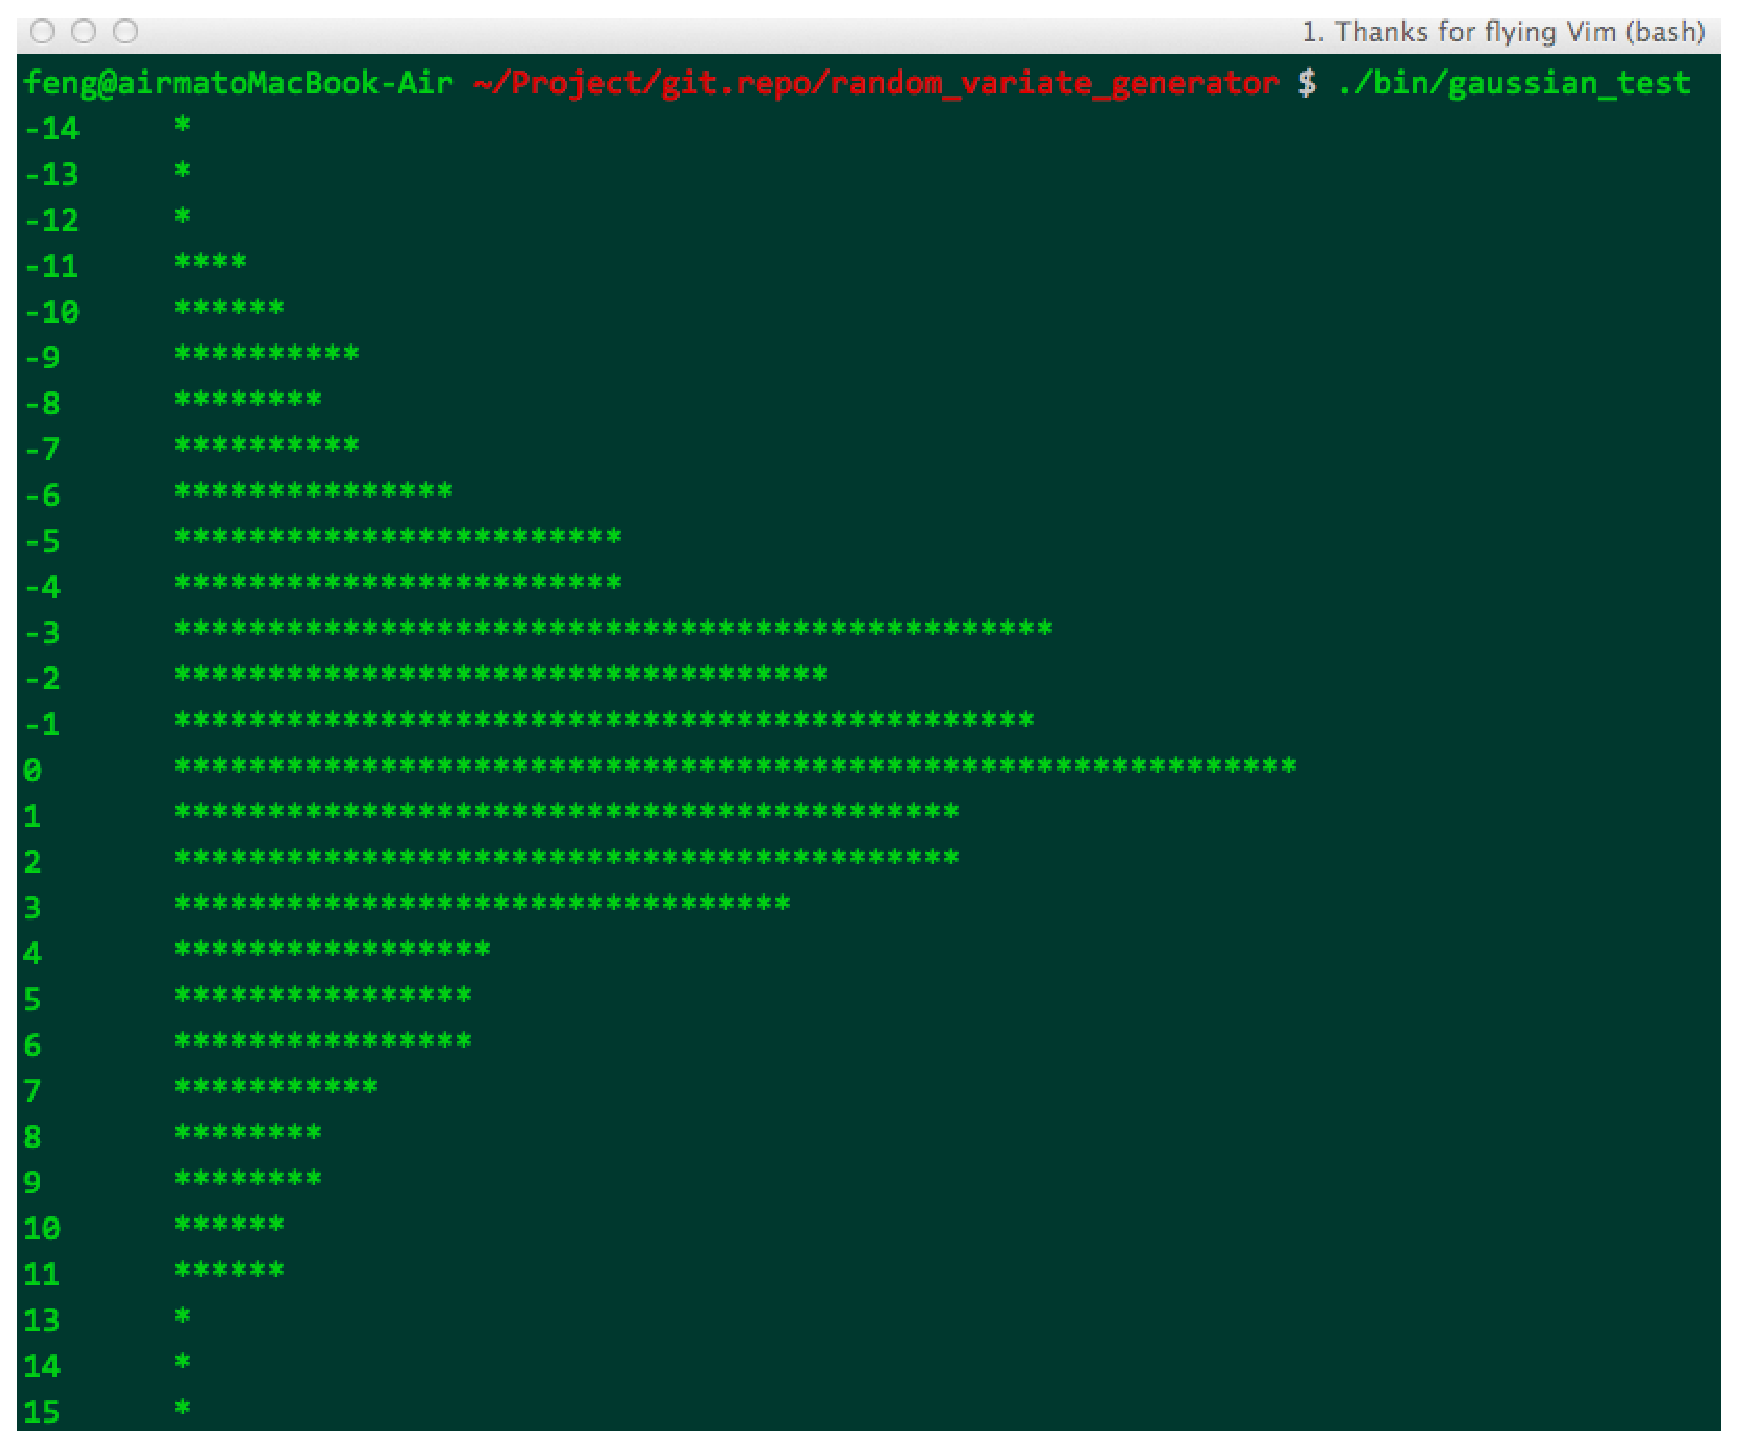
\includegraphics[scale=0.4]{gauss}}
\caption{Gaussian Random Number Example}
\label{fig:gaussian}
\end{figure}

%%code








